%%
\chapter{Introduction}

\section{Background and Motivation}

Atmospheric aerosols play a crucial role in global climate change. They
affect earth's energy budget directly by scattering and absorbing solar and
terrestrial radiation, and indirectly through altering the cloud formation,
lifetime, and radiative properties \citep{Haywood00,Ramanathan01}.
However, quantification of these effects in current climate models is fraught
with uncertainties. The global average of the aerosol effective radiative 
forcing were estimated to range from --0.1 to --1.9 Wm$^{-2}$ with the best 
estimate of --0.9 Wm$^{-2}$ \citep{Boucher13}, indicating that the cooling
effects of aerosol might counteract the warming effects of 1.82$\pm$0.19 
Wm$^{-2}$ caused by the increase of carbon dioxide since the industrial 
revolution \citep{Myhre13}. The climate effects of aerosol particles depend 
on their geographical distribution, optical properties, and efficiency as 
cloud condensation nuclei and ice nuclei. 
Key quantities pertain to the aerosol optical and
cloud-forming properties include particle size distribution (PSD), chemical
composition, mixing state, and morphology \citep{Boucher13}. While the
daily aerosol optical depth (AOD) can be well measured from current satellite
and ground-based remote sensing instrumentations \citep[e.g.,][]{Holben98,Kaufman02},
the accurate quantification of aerosol ERF is in no
small part hindered by our limited knowledge about the aerosol PSD and
refractive index (describing chemical composition and mixing state). 

To fully understand the role of aerosol particles in global climate change, 
further development in observations along with retrieval algorithms for these
aerosol microphysical properties from different platforms are thus highly
needed \citep{Mishchenko04}, and the focus of this two-part series study
is the characterization of aerosol properties from ground-based passive remote
sensing.

\subsection{Previous studies on aerosol microphysical retrievals}

There have been continuous efforts in determining aerosol microphysical
properties from ground-based measurements of direct and/or diffuse solar
radiation since \citet{Angstrom29} first suggested an empirical relationship
between the spectral dependency of extinction coefficients and the size of
aerosol particles. Over thirty years later, \citet{Curcio61} inferred the aerosol
PSD from the spectral particulate extinction coefficients in the visible and
near-infrared regions. Soon with the effective numerical inversion technique
developed by \citet{Phillips62} and \citet{Twomey63} specifically for 
error-involved inverse problem, a number of studies explored the use of either spectral
attenuations or scattered radiances (in a small range of scattering angles) to
determine the aerosol PSD
\citep{Twomey67,Yamamoto69,Dave71,Grassl71,Herman71,King78}.
\citet{Shaw79} and \citet{Nakajima83} were among the first studies that have combined
optical scattering measurements with spectral extinctions to recover particle
size spectrum. \citet{Kaufman94} suggested that useful information is contained
in the sky radiances of larger scattering angles for retrieval of the aerosol
scattering phase function and PSD. The first operational retrieval algorithm
for aerosol microphysical properties was introduced by \citet{Nakajima96},
when the multi-band automatic sun- and sky-scanning radiometer was deployed in
the AErosol RObotic NETwork, or the AERONET \citep{Holben98}. All of
above mentioned methods treated aerosol particles as homogeneous spheres and
with refractive index assumed a priori, even though the refractive index can
highly impact the optical characteristics, especially the scattering 
\citep{Hansen74}. \citet{Tanaka82,Tanaka83} developed an inversion library
method to estimate the complex refractive index and PSD simultaneously from
measurements of scattered radiances polarized in the perpendicular and parallel
directions. Another concept for determining refractive index from both direct
and diffuse angular radiances was developed by \citet{Wendisch94} and 
\citet{Yamasoe98}, which were based on the fact that
sensitivities of scattered radiances to the PSD and those to the refractive
index are dominated on different scattering-angular regions. The current
AERONET operational inversion algorithm was developed by \citet{Dubovik00a},
which has heritage from algorithms developed by \citet{King78} and
\citet{Nakajima83,Nakajima96} but was implemented for simultaneous retrieval of
particle size distribution and complex refractive index with sophisticated
inclusion of multiple a priori constraints. \citet{Dubovik02,Dubovik06} further
implemented the spheroids in the particle shape consideration for desert dust
in the retrieval, and added fractional volume of non-spherical particles to the
inversion products.

\subsection{The AERONET measurements} \label{subsec:cimel318}

With over 400 locations around the word, most AERONET sites are equipped with
an automatic sun and sky scanning spectral radiometer, or the CIMEL CE318 type
SunPhotometer (Figure \ref{fig:cimel318}a), to routinely measure direct and 
diffuse solar radiation in various atmospheric window channels \citep{Holben98}. 
As listed in Table \ref{tab:cimel318} and illustrated in Figure 
\ref{fig:cimel318}, these measurements include direct sun radiances, sky 
radiance on both the solar almucantar and principal planes, as well as the 
optional polarization of sky light on the solar principal plane.

Direct sun radiances at various atmospheric window channels from the
ultra-violet (UV) to near-infrared (NIR) are used to infer the spectral AODs with the
Beer-Lambert-Bouguer Law \citep{Holben98,Smirnov00}. Depending on site-specific
instruments, AOT values are typically reported at 7 wavelengths centered at 340
nm, 380 nm, 440 nm, 500 nm, 675 nm, 870 nm, and 1020 nm. Their calibration
errors are believed to as small as 0.01 for visible and NIR bands and 0.02 for
UV bands.

\begin{figure}[t]
  \centering
  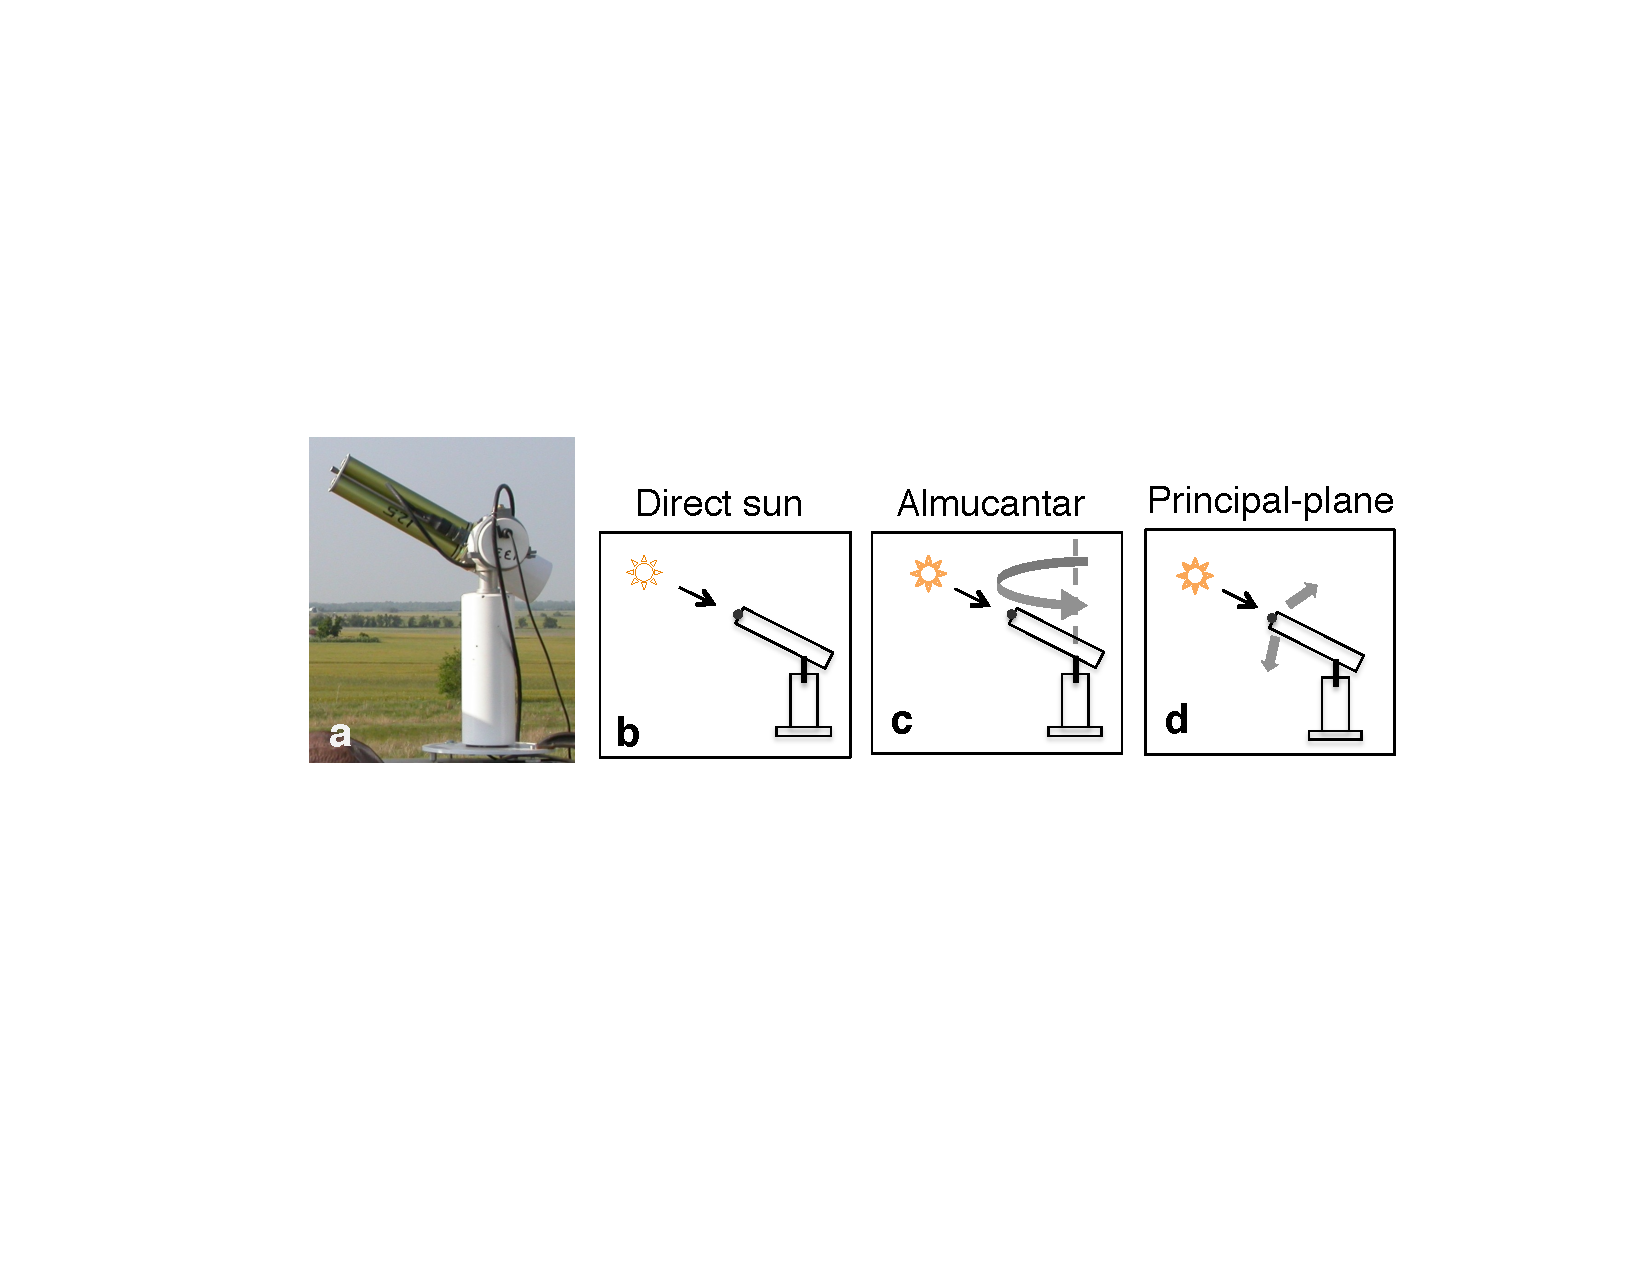
\includegraphics[width={0.95\textwidth}]{figures/cimel318.pdf}
  \caption{A photo of the CIMEL CE318 type SunPhotometer (a) and its 
observational modes: (b) direct-sun radiance scan, (b) sky-radiance scan
on the solar almucantar, (c) solar principal-plane scan for sky radiance
and polarization. Detail scan information are presented in Table
\ref{tab:cimel318} and text.}
  \label{fig:cimel318}
\end{figure}

Sky radiance measurements, which are performed at 440, 670, 870, and 1020-nm
bands with full width spectrum at half maximum (FWHM) of 10 nm, are acquired
from both solar almucantar and solar principal plane. An almucantar is a series 
of measurements taken at the viewing angle of the sun for 76 specified relative 
azimuthal angles (Table \ref{tab:cimel318}). To achieve a wide
enough range of scattering angles, almucantar scans are usually made at an
optical air mass of 1.7 or more (corresponding to solar zenith angle larger
than about 50$^\circ$). The principal-plane sequence for each spectrum performs
right after almucantar scans. It begins with a sun observation, moves 6$^\circ$)
below the sun-ray, sweeps up through the sun, and ends at a scattering angle of
150$^\circ$) or viewing angle achieves horizon, collecting radiances from up to
42 viewing angles. Hereinafter, we will use $\ialm$ and $\ippl$ to represent the sky
radiances from the solar almucantar and solar principal plane, respectively.

\begin{table}[t]
  \centering
  \footnotesize
  \caption{Measurement sequences of the CIMEL CE318 SunPhotometer.}
  \label{tab:cimel318}
  \begin{tabular}{p{5em} p{8em} p{20em} p{6em} }
    \toprule
           & Spectra (nm)& Viewing Geometry ($^\circ$)& Applications \\ 
    \midrule
    Direct sun & 340--1020 \newline 340--1640\textsuperscript{a} & Target to
the sun & AOD, \newline $P_\text{w}$, AE \\
    \hline
    Almucantar ($\ialm$)& 440, 675, 870, 1020 \newline (340, 380, 500,
1640)\textsuperscript{a} & Azimuth angles relative to
Sun: 6, 5, 4.5, 4, 3.5, 3, 2.5, 2, --2, --2.5, --3, --3.5, --4, --4.5, --5, --6,
--8, --10, --12, --14, --16, --18, --20, --25, --30, --35, --40, --45, --50,
--60, --70, --80, --90, --100, --110, --120, --130, --140, --160, --180
(Duplicate above sequence for a complete counter clockwise rotation to --6) & 
PSD, \newline $\mreal$, $\mimag$, \newline SSA, \newline phase function\\
    \hline
    Principal-plane ($\ippl$)& Same as above & Scattering angle from
Sun: --6, --5, --4.5, --4, --3.5, --3, --2.5, --2, 2, 2.5, 3, 3.5, 4, 4.5, 5,
6, 8, 10, 12, 14, 16, 18, 20, 25, 30, 35, 40, 45, 50, 60, 70, 80, 90, 100, 110, 
120, 130, 140 (negative is below the Sun) & Same as above \\
    \hline
    Polarization ($\ipp, \dolppp$) & 870, \newline (340, 380, 440, 500, 675, 870, 1020,
1640)\textsuperscript{a} & Zenith angle on the
solar principal plane: --85, --80, --75, --70, --65, --60, --55, --50, --45,
--40, --35, --30, --25, --20, --15, --10, --5, 5, 10, 15, 20, 25, 30, 35, 40, 
45, 50, 55, 60, 65, 70, 75, 80, 85 (negative is in the anti-solar direction) &
Not used yet \\
    \bottomrule
     \multicolumn{4}{m{35em}}{\textsuperscript{a}Additional measurements taken
by the newer-generation CIMEL-318DP SunPhotometer.}
  \end{tabular}
\end{table}

These sky radiance data are used in the current AEROENT operational inversion
algorithm \citep{Dubovik00a,Dubovik06} (hereafter Dubovik00\&06) to derive: 
(1) the aerosol particle size distribution (PSD) in
terms of the aerosol volume (in the atmospheric column) at 22 size bins, (2)
the fractional volume of non-spherical particles, and (3) the complex
refractive index assumed to be independent of particle size. From
those microphysical parameters, the \Dub algorithm computes the aerosol
single scattering albedo (SSA) and the phase function. Uncertainties in
the AERONET inversion products are 15--100\% for the bin-based PSD parameters,
0.025--0.05 for real-part refractive index and 0.03 for SSA \citep{Dubovik00b}.

Light polarization measurements are performed optionally over many sites. They
are measured by the SunPhotometer with three polarizers placed
60$^\circ$ between each axial direction. The total radiance is derived by 
\begin{equation}
\ipp = \frac{2}{3}\left( I_1+I_2+I_3 \right),
\end{equation}
where $I_1$, $I_2$, and $I_3$ are radiance with these three polarizers,
respectively. The degree of linear polarization (DOLP) of skylight is inferred
by
\begin{equation}
\dolppp = \frac{2(I_1^2+I_2^2+I_3^2-I_1I_2-I_2I_3-I_1I_3)^(1/2)}{I_1+I_2+I_3}.
\end{equation}
It should be noted that we prefer to use $\dolppp$ instead of polarized radiance
in our inversion, since as a relative quantity it is more accurate.
Polarization measurements are made every hour (right after principal plane
scans) at 870 nm in the principal plane at 5$^\circ$ increments between viewing zenith
angle of $-85^\circ$ and $+85^\circ$. These measurements are optional depending on the
instrument version and configuration, and are currently available mostly over
European and African stations. Recently, multi-spectral polarizations have also
been taken with a newer-generation SunPhotometer (CIMEL CE318-DP) at some sites
\citep{Li09} and the UAE$^2$ fields campaign \citep{Reid08}. Here we
focus our study on using multi-spectral polarizations for the inversion of
aerosol parameters.

\subsection{Challenges and opportunities}

While the AERONET AOD and other inversion products have been widely used to
study the climatology of aerosol optical properties \citep{Dubovik02b,Levy07a}
and for the development and validation of aerosol retrieval
algorithms for satellite sensors such as the Moderate Resolution Imaging
Spectrometer (MODIS) \citep{Kaufman97,Remer05,Levy07b,Levy10,Wang10}
and the Multi-angle Imaging SpectroRadiometer
(MISR) \citep{Diner98,Kahn10}, the AERONET operational
algorithm also faces: (i) challenges in evaluation of aerosol data either
retrieved from newer-generation satellite sensors or simulated from chemistry
transport models, and (ii) opportunities to improve the retrieval through the
use of multi-spectral polarization measurements that are now available at a few
sites and will be made available at more sites as part of the AERONET future
research development (\url{http://aeronet.gsfc.nasa.gov}). These challenges and
opportunities, as further described below, are also the motivation for us to
develop a new research algorithm.

The first challenge is that newer-generation satellite sensors are expected to
offer aerosol microphysical products with accuracy that is equivalent to, if
not higher than, that of the current AERONET microphysical products. For
instance, the Aerosol Polarimetry Sensor (APS) for the NASA Glory mission,
through measuring the first three Stokes vector elements simultaneously from
250 viewing angles at nine spectral bands (410, 443, 556, 670, 865, 910, 1370,
1610, and 2200 nm), was designed to retrieve aerosol effective radius ($\reff$),
effective variance ($\veff$), and spectral complex index of refraction for both
fine and coarse modes \citep{Mishchenko07}. While no actual product is
available because of the failure of Glory launch, several case studies with the
APS's prototype airborne sensor, RSP (the Remote Sensing Polarimeter),
demonstrated feasibility of APS algorithm \citep{Chowdhary02,Chowdhary05,
Mishchenko04,Waquet09}. At least in the case of
spherical particles, the accuracy of APS’s bi-modal aerosol products was
expected to be 10\% for $\reff$, 40\% for $\veff$, 0.02 for $\mreal$, and 0.03 for the SSA
($\assa$) \citep{Mishchenko07}. Some of these accuracy expectations are
unlikely to be matched by existing ground-based and in situ instruments,
including those at the AERONET sites. Moreover, the current AERONET retrieval
of the refractive index and the $\assa$ are not recommended to use when the 440-nm
AOD is lower than 0.4 \citep{Holben06} due to expected limited accuracy
identified in the detailed sensitivity study by \citep{Dubovik00b}.

The second challenge is associated with the inconsistency in assumptions of PSD
that exists between current AERONET inversion products and satellite retrievals
on the one hand, and the aerosol models used by climate models on the
other hand. Specifically, the \Dub algorithm retrieves the aerosol PSD
on in 22 discrete size bins. In contrast, a continuous PSD function (e.g.,
lognormal) is usually assumed in satellite retrieval algorithms, such as those
for APS/RSP \citep{Mishchenko07, Waquet09} and the
POLDER/PARASOL algorithm \citep{Hasekamp11}. Also, aerosol microphysical
properties are usually calculated with continuous PSD assumptions in many
chemistry transport models, such as GEOS-Chem \citep{Drury10, Wang10}
and the GOCART model \citep{Chin02}. Clearly, the actual aerosol PSD
is never a perfect lognormal distribution, but neither is it discrete. At least
from the scattering perspective, the aerosol PSD can be well characterized with
an effective radius $\reff$ and an effective variance $\veff$, while the specific
function of the PSD is shown to be much less important \citep{Hansen74}.
In other words, since the retrieval is based on the information content
in the particle optical scattering, the most relevant size parameters,
regardless of the PSD shape, should be $\reff$ and $\veff$, at least for spherical
particles.

The third challenge is that the assumption of a size-independent refractive
index (and SSA) in \Dub is not in line with the majority of counterpart
satellite retrieval algorithms \citep[e.g.,][]{Mishchenko07, Hasekamp11,
Martonchik09}, which often uses different refractive indices
for various individual aerosol modes. In many cases, tropospheric aerosol is a
mixture of modes with substantially different refractive indices. For example,
smoke from biomass burning can be mixed with mineral dust over western coastal
North Africa \citep{Yang13}. Furthermore, the assumption of
size-independent refractive index can lead to errors in the retrieval of the
size distributions when the refractive indices for fine- and coarse-mode
aerosols differ substantially \citep{Dubovik00b, Chowdhary01}.
Thus, a mode-resolved parameterization of the refractive index in an aerosol
retrieval algorithm not only can facilitate the validation of satellite
products and chemistry transport models, but also is expected to improve the
accuracy of PSD and SSA retrievals for each mode. \citep{Dubovik00b} have
tested the possibility of retrieving separated refractive indices of fine and
coarse modes, however, they concluded that the retrieval of bi-modal refractive
indices is essentially non-unique due to limited information in the AERONET
radiance-only observations. 

Therefore, this work aims to developing an algorithm to retrieve the aerosol
microphysical properties of both fine and coarse aerosol modes,
which embraces the future opportunities of
deploying polarization measurements through AERONET, and ameliorates the
aforementioned limitations in the \Dub algorithm by incorporating both
radiance and polarization data. Polarization measurements contain valuable
information on aerosol microphysical properties \citep{Mishchenko97},
as the polarization of the scattered light is highly sensitive to aerosol size
and refractive index \citep{Hansen74, Mishchenko02}. We note, however, their
conclusions were based on consideration of
spherical aerosol particles and were primarily from a theoretical point of
view. In contrast, the studies by \citet{Dubovik06} and \citet{Deuze93,
Deuze01} revealed serious limitation of polarimetric retrieval of the properties
for the coarse mode, especially non-spherical aerosols. Moreover, \citet{Dubovik06}
have shown that while the polarimetic observation of fine particles and large
spheres are highly sensitive to the real part of refractive index, even they have
non-negligible sensitivity to particle shape. Therefore, adding polarization
measurements to the inversion has great potential to improve the accuracy of
AERONET microphysical retrievals, provided that the difficulty of representing
aerosol particle shapes is recognized or adequately addressed. In these
regards, most of the past efforts seem to suggest clear improvements in
characterization of fine mode aerosol using polarimetric observations. For
example, \citet{Li09}, based upon the \Dub algorithm, demonstrated
the possibility to reduce errors in the fine-mode size distribution, real part
of the refractive index, and particle shape parameters. 

\section{Research Goals and Thesis Outline} \label{sec:objective}

As discussed above, this dissertation seeks to contribute an improved
research algorithm that retrieves aerosol microphysical properties from AERONET
measurements of light radiance and polarization, with emphasis on elucidating
the potential value of polarization measurements. It does so by 
pursuing the following three objectives:

\begin{enumerate}
\item \textit{Develop ground-based inversion algorithms for the
retrieval of aerosol refractive indices and particle size distribution from a 
combined use of direct and diffuse solar radiation measurements from AERONET.}
\newline
Retrieving aerosol information from remote sensing observation
involves two type of development, i.e., the forward modeling and inverse
modeling. In Chapter \ref{ch:model}, I present a unified radiative transfer 
model---UNL-VRTM---that we have developed specifically for inversion of
aerosol properties from remote sensing measurements \citep{Wang14}. The
key feature of UNL-VRTM is that it not only simulates the
polarimetric radiation in the atmosphere but also, more importantly,
can compute the analytical derivatives of these radiation fields with respect
to aerosol microphysical parameters. In the subsequent chapter, I
describe an inversion algorithm that is developed by integrating the UNL-VRTM 
with statistically optimization approach to retrieve 22 aerosol
microphysical parameters from the AERONET measured multi-spectral and
multi-angular light radiance and polarization. 

\item \textit{Conduct a sensitivity study and error budgeting exercise to
characterize retrieval accuracy and error sources.} 
\newline 
In order to explore the potential of the AERONET polarization measurements
for improving aerosol microphysical retrieval, our inversion testbed is
used to examine the information content of these measurements with and without
radiation in the Chapter \ref{ch:info}. The analysis focuses on
how the added polarization measurements impact on the retrieval accuracy
the in aerosol particle size distribution, spectral refractive
index, and single scattering albedo. We also investigate the how the 
added polarization measurements can reduce the retrieval error for these
properties.  

\item \textit{Perform ground-based retrievals using available AERONET
polarimetric measurements.}
\newline
In Chapter \ref{ch:case}, I applied our new research algorithm to a suite of
photo-polarimetric measurements taken from the new-generation SunPhotometer
at the Beijing\_RADI AERONET station. In order to demonstrate the value of 
adding polarization measurements, we performed aerosol retrievals from 
radiance measurements only, in addition to the retrievals using both radiance 
and polarization measurements. 
\end{enumerate}
